\documentclass{article}
\usepackage[utf8]{inputenc}

\usepackage[T1]{fontenc}
\usepackage[swedish]{babel}
\usepackage[makeroom]{cancel}
\usepackage{amssymb, amsmath, lmodern, units, icomma, color, graphicx, bbm, hyperref, pdfpages, csquotes}
\usepackage[backend=biber]{biblatex}

\setlength{\parindent}{0em}
\setlength{\parskip}{0.5em}

\addbibresource{referenser.bib}

\begin{document}

\begin{titlepage} \newcommand{\HRule}{\rule{\linewidth}{0.3mm}}
\center
\textsc{\Large Chalmers tekniska högskola}\\[0.05cm] % Name of your university/college \textsc{\normalsize Teknisk Matematik}\\[0.2cm]
%\normalsize \\ % Major heading such as course name
\normalsize \today

\HRule \\[0.08cm]
{ \large Planeringsrapport \\ \normalsize{-- Programmering som undervisningsverktyg för signaler och system}}\\[0.08cm] %Signalteori är för stort?
\HRule \\[0.3cm]

\vfill

\begin{flushleft} \small
    \emph{Author: \\
    \quad Filip Lindahl\\
    \quad Cecilia Rosvall\\
    \quad Peter Ngo\\
    \quad Jacob Jonsson\\
    \quad Joakim Olsson\\}
\end{flushleft}
\end{titlepage}
\newpage
\tableofcontents
\newpage

\section{Bakgrund}
På Chalmers Tekniska Högskola har det funnits en lång trend
där studenterna på utbildningen för Datateknik har haft
svårigheter med kurserna \textit{Transformer, Signaler och System},
hädanefter omnämnd som ''TSS'', och \textit{Reglerteknik}.
Dessa svårigheter tror examinatorerna i kurserna beror till
stor del på att studenterna inte är tillräckligt bekväma
i det matematiska språket.
Studenterna på Datateknik har inte tillräcklig vana att
tolka innebörden av de matematiska beskrivningarna och är
allmänt ovana vid matematiskt hantverk.
Därför lägger datastudenterna det mesta av sin energi
på att få ihop matematiken rent praktiskt,
istället för att se vad matematiken står för.

Detta syns bland annat i statistiken för hur många
datastudenter som klarar kurserna, under perioden från
2010 till 2016 blev i genomsnitt 51\% av alla som skrev
tentamen godkända i TSS och under samma period blev
53\% godkända i Reglerteknik \cite{tentastatistik}.
Det finns även ett mörkertal i dessa siffror eftersom
inte alla studenter skriver tentan, exempelvis
valde 48 studenter utav 122 registrerade att inte
tentera Reglerteknik 2014 \cite{kursinformation:ere102:14-15}.

För att minska svårigheterna som studenterna har för dessa kurser
påbörjades ett pedagogiskt projekt, DSLsOfMath, som hittills
resulterat i kursen \textit{Matematikens domänspecifika språk}, där man
använder funktionell programmering för att beskriva matematiska problem \cite{kursplan:dslsofmath}.
Resonemanget bakom detta var att funktionell programmering är ett
verktyg som datastudenterna har erfarenhet av och som använder en
notation med fokus på tydlighet som lämpar sig relativt väl för
att lära ut matematiska begrepp \cite{tfpie}.

Detta projekt uppstod som en avgrening av DSLsOfMath-projektet med
fokus mer på signal- och systemteoretiska färdigheter snarare än
en allmän matematisk grund.

\section{Syfte}
Syftet med projektet är att underlätta för studenter inom datateknik
att ta till sig signal- och systemteoretiska ämnen genom att utnyttja
deras kunskaper inom programmering och även göra det möjligt att
betrakta ämnet ur en programmerares perspektiv.
Med detta hoppas man göra gapet mellan datateknik och
signalteori mindre och minska problemen som nämns i
bakgrundsavsnittet.

Projektet är tänkt att resultera i en handledningsguide, en så kallad
tutorial, som kan fungera som ett komplement till de kurser som ges
inom signalteori på den datatekniska grundutbildningen. Denna guide ska innehålla förklaringar och programmeringsövningar som är anpassade för studenter på den datatekniska utbildningen.

\section{Problemanalys}
Uppgiften i detta projekt kommer bestå i att utarbeta en tutorial som
komplement till kurserna “Reglerteknik” och “Transformer, signaler och
system”.

För att kunna utveckla denna produkt kommer först omfattande
förstudier behöva bedrivas innan vi utvecklar vår produkt och denna
produkt kommer sedan behöva testas.

\subsection{Förstudier}
För att komma till rätta med datastudenternas största svårigheterna
med förståelsen inom ämnena behöver vi först undersöka var dessa
svårigheter ligger mer i detalj.

Dessutom kommer vi även behöva bedriva en hel del efterforskningar
och litteraturstudier inom såväl pedagogik som de signalteoretiska
ämnen vi beskriver för att kunna skriva en produkt med korrekt och
tydligt innehåll.

\subsection{Produkten}
Efter förstudierna kommer en tutorial utvecklas.
%
Innehållet i denna kommer bestå av förklarande teori,
exempel inom såväl teori som programmering, samt övningar
med tillhörande lösningar.

\subsection{Testa produkten}
Produkten kommer sedan behöva testas på den aktuella målgruppen för
möjligheten att uppdatera och förbättra den slutgiltiga produkten.

\section{Avgränsning}
I denna projekt skrivs en handlednings guide vars avsikt är att
förtydliga de delar studenter inom datateknik finner svårt i kurserna
“Transform, Signal och System” och “Reglerteknik”.
%
Detta innebär att vi endast fokuserar på svårigheter inom dessa kurser
och inte ett alternativt läromaterial som täcker hela själva ämnet.
%
Det vill säga, produkten kommer inte bli ett underlag för motsvarande
kurs DAT325 utan ett komplement till kurserna SSY080 och ERE103.

\section{Metod}
\subsection{Förstudier}
För att samla in information om vilka moment i kurserna
TSS och Reglerteknik som datastudenter har svårast för har
vi intervjuat examinatorerna om de övergripande
svårigheterna inom båda kurserna.
Vi kommer under projektets gång ha fler intervjuer med
examinatorerna där det läggs mer fokus på detaljer.

För att få information av datastudenterna om vad de tyckte
var svårt kommer vi utarbeta en enkät om såväl kurserna
som deras förkunskaper och analysera resultatet från denna.

För att kunna skriva en lättläst och begriplig tutorial
kommer vi studera litteratur inom pedagogik samt
alternativa inlärningsformer som exempelvis boken och
hemsidan \textit{Learn you a Haskell for great good} \cite{learnyouahaskell}.
Litteraturen kommer väljas baserat på rekomendationer från
projektets handledare och anställda vid Chalmers bibliotek
samt egna efterforskningar.
%Referens!

\subsection{Produkten}
Programeringskoden till projektet kommer skrivas i Haskell,
vilket från början var specifierat från instutitionen för
Data och Informationsteknik som skapade projektet.
Haskell är ett programeringsspråk med syntax som liknar den
matematiska notationen. Språket har dessutom egenskaper
som gör att det lämpar sig väl som värdspråk för ett domänspecifikt språk,
Haskell har till exempel stöd för att skapa egna datatyper.
Därför såg vi ingen anledning att ändra specifikationen.

Rent strukturellt planerar vi att dela upp vår tutorial i
sex delavsnitt som kommer att innehålla informativ text som
förklarar delavsnittet och runt 15 -- 20 uppgifter vardera.
I uppgifterna får studenterna lära sig om signaler och
system genom att implementera de inblandade typerna
och relationerna som domänspecifika språk i Haskell.

\subsection{Testa produkten}
För att testa svårighetsgraden på vår produkt kommer vi
först att testa vår tutorials övningar internt. Tanken är att
vi kommer dela upp delavsnitten så att två till tre personer
skriver ett delavsnitt och sedan kan gruppmedlemmarna testa
varandras arbete. På detta sätt kommer vi ha möjlighet att
förbättra och utveckla delavsnitten innan de
testas på andra studenter.

Sedan kommer vi att testa vår tutorial på datastudenter genom
att de får läsa texterna och göra uppgifter till ett eller flera avsnitt.
Efter att de har läst och implementerat uppgifterna kommer de att få svara på
frågor angående hur de upplevde texten och uppgifter i en enkät.
I enkäten kommer vi också att testa studenternas förståelse av det avhandlade avsnittet.

Utifrån dessa tester och enkäter kommer vi sedan vidareutveckla och förfina slutprodukten.

\section{Tidsplan}
För att göra projektet mer överskådligt ur ett
tidsperspektiv har ett antal milstolpar tagits fram.
Samtliga av dessa har en preliminär deadline för
att ge gruppen något att arbeta mot.

\subsection{Milstolpar}
\begin{itemize}
 \item 2016-02-10 - Planeringsrapport och grov planering klar
 \item 2016-02-11 - Fackspråkshandledningstillfälle 1
 \item 2016-02-12 - Planeringsrapport inlämning
 \item 2016-02-24 - Intervjuer, grundläggande efterforskningar om TSS och reglerkurserna klara
 \item 2016-02-24 - Litteraturstudier inom pedagogik klara
 \item 2016-03-01 - Utkast för grov tutorial klar (uppgifter ej klara)
 \item 2016-03-01 - Få klart ett litet avsnitt för halvtidsredovisningen, med förslag på uppgifter och text
 \item 2016-03-01 - Halvtidsredovisning
 \item 2016-03-15 - Uppgifter och utkast till text för två av sex delavsnitt i tutorial klara
 \item 2016-03-22 - Första utkast till rapporten klart
 \item 2016-03-22 - Fackspråkshandledningstillfälle 2
 \item 2016-03-28 - Bearbetning av feedback från fackspråk
 \item 2016-04-11 - Uppgifter och utkast till text för fyra av sex delavsnitt i tutorial klara
 \item 2016-04-25 - Uppgifter och utkast till alla delavsnitt i tutorial klara
 \item 2016-04-27 - Eventuell engelsk (forskningsinriktad) uppsats klar
 \item 2016-04-28 - Andra utkast till rapporten klart
 \item 2016-05-04 - Tutorial klar och testad
 \item 2016-05-11 - Rapporten klar
 \item 2016-05-13 - Fackspråkshandledningstillfälle 3
 \item 2016-05-16 - Rapportinlämning
 \item 2016-05-17 - Utställning
 \item 2016-05-26 - Deadline för opposition
 \item 2016-05-26/27 - Slutredovisning
 \item 2016-06-01 - Sista inlämningen
\end{itemize}

\newpage
\subsection{Gantt schema}
Nedan följer ett Gantt schema för att ge en överblick om hur gruppens arbete fördelas över projekttiden.
\begin{figure}
    \centering
    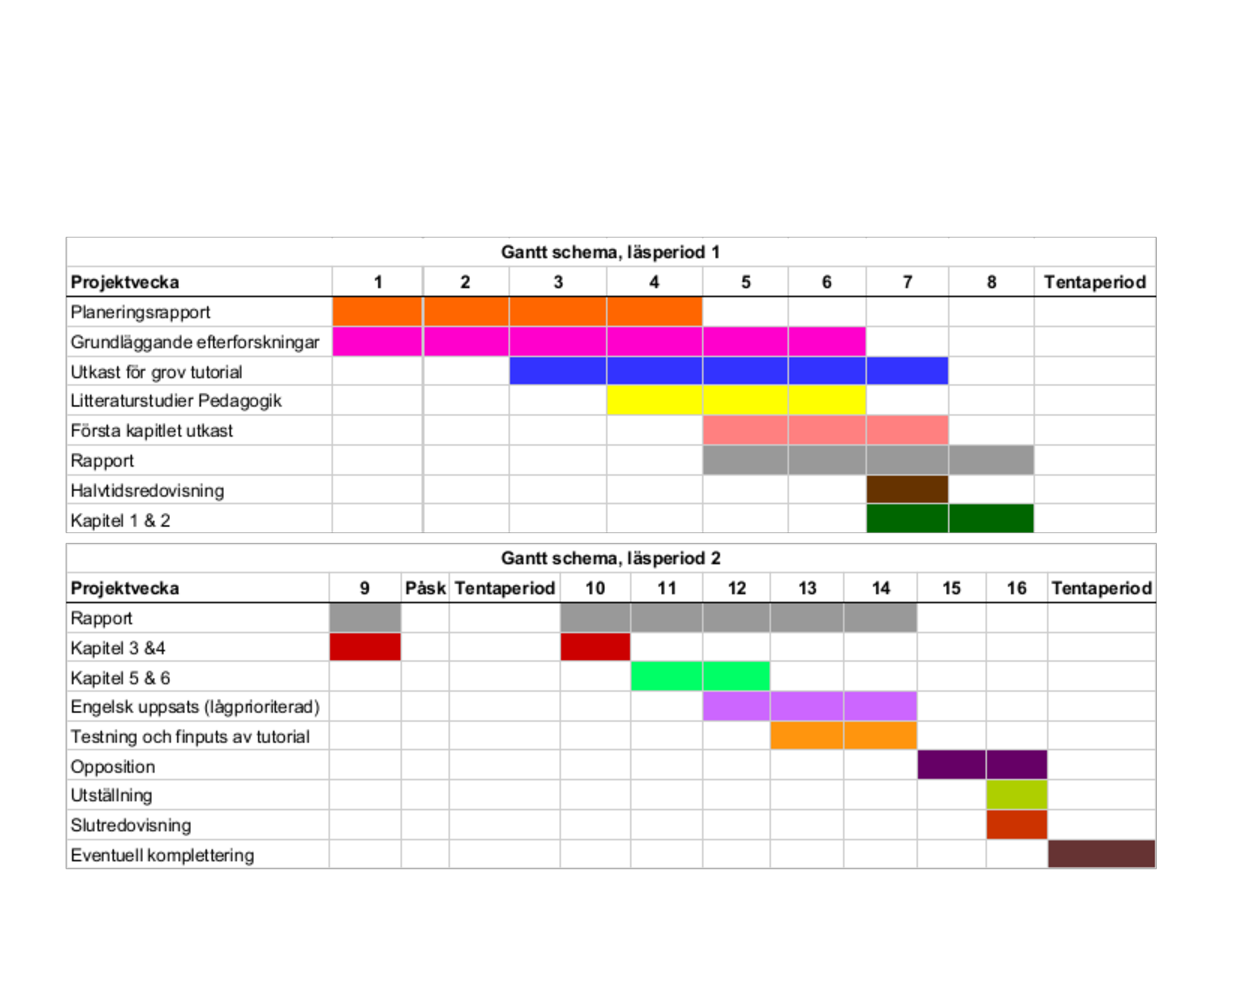
\includepdf[width=0.8\paperwidth]{gantt}
\end{figure}
\newpage

\printbibliography
\end{document}
